% Sync test talk: every element kind the converter handles, with the edits an AI author
% typically makes to a talk marked by docstrip-like guards. build.py writes one plain .tex per
% variant (tests/decks/sync/out/<variant>.tex) and compiles it:
%   %<flag> line        the rest of the line only when the flag is set
%   %<!flag> line       the rest of the line only when the flag is not set
%   %<*flag> ... %</flag>, %<*!flag> ... %</!flag>   the same for blocks of lines
\documentclass[aspectratio=169]{beamer}
\usetheme{Madrid}
\setbeamertemplate{navigation symbols}{}
%<retheme>\setbeamerfont{frametitle}{size=\huge}
%<retheme>\setbeamercolor{frametitle}{bg=red!20, fg=red!50!black}
\setbeameroption{show notes}
\usepackage{amsmath,amssymb,booktabs}
\usepackage{tikz}
\usetikzlibrary{tikzmark,positioning,arrows.meta}
\newcommand{\circled}[1]{\tikz[baseline=(c.base)]\node[circle,draw,inner sep=1pt](c){#1};}

\title[Deck sync]{Keeping Slides and Source in Sync}
\subtitle{Three-way merges for converted decks}
\author[A.~Author]{Alice Author}
\institute[Uni]{University of Examples}
\date{September 2026}

\begin{document}

\begin{frame}[label=title]
  \titlepage
\end{frame}

%<!retitle>\begin{frame}[label=motivation]{Why decks and sources diverge}
%<retitle>\begin{frame}[label=motivation]{Why decks drift away from their source}
  \begin{itemize}
%<!reword>    \item The source is written in \LaTeX{} by an author and converted once
%<reword>    \item The source is written in \LaTeX{} by an AI assistant and converted once
    \item People polish the converted deck by hand
      \begin{itemize}
        \item fixing typos and wording
%<!removebullet>        \item moving pictures around
        \item adding their own slides
      \end{itemize}
    \pause
    \item Later the source changes again
%<addbullet>    \item Converting again would throw away every manual edit
  \end{itemize}
%<!notes>  \note{Start with the story: one author, many editors.}
%<notes>  \note{Start with a show of hands: who edited a converted deck?}
\end{frame}

\begin{frame}[label=steps]{The sync algorithm}
  \begin{enumerate}
    \item Read the base snapshot
    \item Convert the new source
%<numbers>    \item Match slides by their frame labels
    \item Read the live deck
%<!numbers>    \item Merge and write the changes
%<numbers>    \item Merge the changes and write them back
  \end{enumerate}
\end{frame}

\begin{frame}[label=merge]{Merging text}
  A deck edit and a source edit to the same paragraph are merged word by word. The merge
%<!formula>  is clean when the changed words don't overlap, and the distance $\bar{d}_t^{(k)}$ counts
%<formula>  is clean when the changed words don't overlap, and the distance $\hat{\delta}_{t+1}^{(k)}$ counts
  the words both sides changed since the last sync.

  \medskip
  Step \circled{2} then writes the merged paragraph back into the deck.
\end{frame}

\begin{frame}[label=convergence]{Convergence}
  \begin{columns}[c]
    \column{0.55\textwidth}
    \begin{tikzpicture}[scale=0.9]
      \draw[->] (0,0) -- (5.4,0) node[right] {\small syncs};
      \draw[->] (0,0) -- (0,3.3) node[above] {\small open conflicts};
%<!figure>      \draw[very thick, blue] plot[smooth, domain=0:5] (\x, {2.8*exp(-0.45*\x)});
%<figure>      \draw[very thick, red!80!black] plot[smooth, domain=0:5] (\x, {3*exp(-1.1*\x)});
%<figure>      \draw[dashed, gray] (0,1) -- (5,1);
    \end{tikzpicture}
    \column{0.4\textwidth}
    Conflicts disappear once the source says what the deck says.
  \end{columns}
\end{frame}

%<*!reorder>
\begin{frame}[label=policy]{Merge policy}
%<!blockedit>  \begin{block}{Deck edits win}
%<blockedit>  \begin{block}{Deck edits come first}
%<!blockedit>    A source change to a field the deck also edited is reported as a conflict.
%<blockedit>    A source change to a field the deck also edited is kept aside and listed as a conflict.
  \end{block}
  \vspace{1em}
  Both versions go into the report.
\end{frame}

%</!reorder>
\begin{frame}[label=results]{Results}
  \centering
%<tablemove>  Measured on the sync test talk.\par\bigskip
  \begin{tabular}{lrr}
    \toprule
    Scenario & Edits kept & Time \\
    \midrule
%<!tablecell>    Disjoint & 100\% & 3.9 s \\
%<tablecell>    Disjoint & 100\% & 4.7 s \\
    Same element & 100\% & 5.1 s \\
    Conflicts & 92\% & 6.0 s \\
%<tablerow>    Deletions & 100\% & 4.2 s \\
    \bottomrule
  \end{tabular}
\end{frame}

%<*reorder>
\begin{frame}[label=policy]{Merge policy}
%<!blockedit>  \begin{block}{Deck edits win}
%<blockedit>  \begin{block}{Deck edits come first}
%<!blockedit>    A source change to a field the deck also edited is reported as a conflict.
%<blockedit>    A source change to a field the deck also edited is kept aside and listed as a conflict.
  \end{block}
  \vspace{1em}
  Both versions go into the report.
\end{frame}

%</reorder>
%<*addframe>
\begin{frame}[label=pull]{Pulling edits back}
  \begin{columns}[c]
    \column{0.6\textwidth}
    \begin{itemize}
      \item Deck edits are listed with their source lines
      \item Plain wording edits are patched into the source
    \end{itemize}
    \column{0.35\textwidth}
    \centering
    
\begin{tikzpicture}
      \draw[thick, teal] (0,0) rectangle (1.6,1.1);
      \draw[thick, orange] (2.2,0) rectangle (3.8,1.1);
      \draw[->, very thick, gray] (2.1,0.55) to[bend right=40] (1.7,0.55);
    \end{tikzpicture}
  \end{columns}
\end{frame}

%</addframe>
%<*!deleteframe>
\begin{frame}[label=versions]{Three versions}
  \centering
  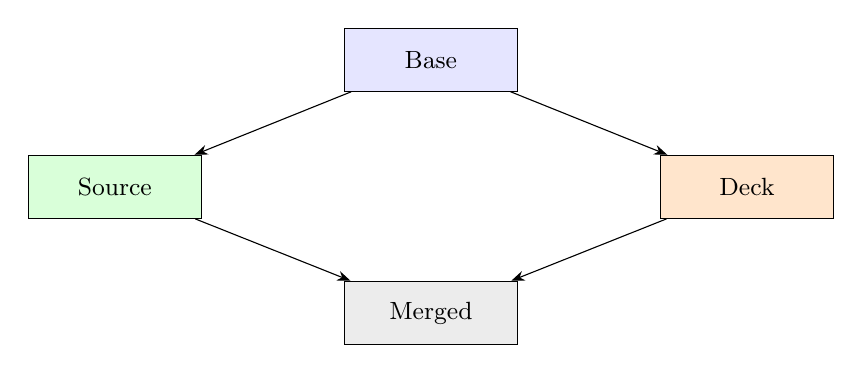
\begin{tikzpicture}[node distance=0.8cm and 1.8cm, every node/.style={font=\small}]
    \node[draw, fill=blue!10, minimum width=2.2cm, minimum height=0.8cm] (base) {Base};
    \node[draw, fill=green!15, minimum width=2.2cm, minimum height=0.8cm, below left=of base] (ours) {Source};
    \node[draw, fill=orange!20, minimum width=2.2cm, minimum height=0.8cm, below right=of base] (theirs) {Deck};
    \node[draw, fill=gray!15, minimum width=2.2cm, minimum height=0.8cm, below=2.4cm of base] (merged) {Merged};
    \draw[-{Stealth}] (base) -- (ours);
    \draw[-{Stealth}] (base) -- (theirs);
    \draw[-{Stealth}] (ours) -- (merged);
    \draw[-{Stealth}] (theirs) -- (merged);
  \end{tikzpicture}
\end{frame}

%</!deleteframe>
\begin{frame}[label=identity]{Finding the same slide}
  Every frame gets a \tikzmarknode{lab}{label} in the source, so a slide keeps its identity
  when its title changes, when the frames move around or when a new frame comes before it:
  the \tikzmarknode{key}{key} stays the same.
  \begin{tikzpicture}[remember picture, overlay]
    \draw[->, red, thick] (lab.south) to[out=-90, in=90] (key.north);
  \end{tikzpicture}
%<!notes>  \note{Labels are the stable key; titles are only a fallback.}
%<notes>  \note{Labels are the stable key. Titles and page numbers are only fallbacks.}
\end{frame}

%<!untitled>\begin{frame}{Conclusions}
%<untitled>\begin{frame}{Takeaways}
  \begin{itemize}
    \item Deck edits survive every sync
    \item Conflicts are reported with both versions
  \end{itemize}
\end{frame}

%<*probes>
\begin{frame}[label=grow,t]{Room to grow}
%<probepush>  \vspace*{1.5em}
%<!probereword>  The person writes a longer version of this paragraph than the converter
%<probereword>  The person types a longer version of this paragraph than the converter
  made room for, so its box has to grow downwards.

  \medskip
  \centering
  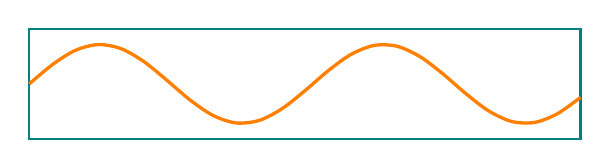
\begin{tikzpicture}
    \draw[thick, teal] (0,0) rectangle (7,1.4);
    \draw[very thick, orange] plot[smooth, domain=0:7] (\x, {0.7+0.5*sin(\x*100)});
  \end{tikzpicture}
\end{frame}

\begin{frame}[label=twoboxes,t]{Two boxes}
%<probepush>  The source adds this line above both boxes.\par\medskip
  The first box holds two lines of text, written so that it wraps once at the
  right margin of the frame.

  \medskip
  \hspace*{2cm}\parbox{7cm}{The second box stands below it, indented, on its own.}
\end{frame}

\begin{frame}[label=display,t]{Display math}
%<probepush>  The source adds this line above the equation.\par\medskip
  The equation below stands between two paragraphs:
  \[ \sum_{k=1}^{n} \frac{d_k^2}{\sigma_k} = \int_0^1 f(x)\,dx \]
  and this paragraph comes after it.
\end{frame}

%</probes>
\end{document}
